\section{Circle and Rectangle}


 \subsection{Image Description}

  \begin{itemize}
     \item Image size: $1200 \times 1000$ pixels
     \item Surface area of shapes: $90000$ pixels
     \item The centroid of the shape is located at the center of the image
  \end{itemize}



 \subsection{Output Analysis}
 
   \begin{figure}[h!]
     \centering
     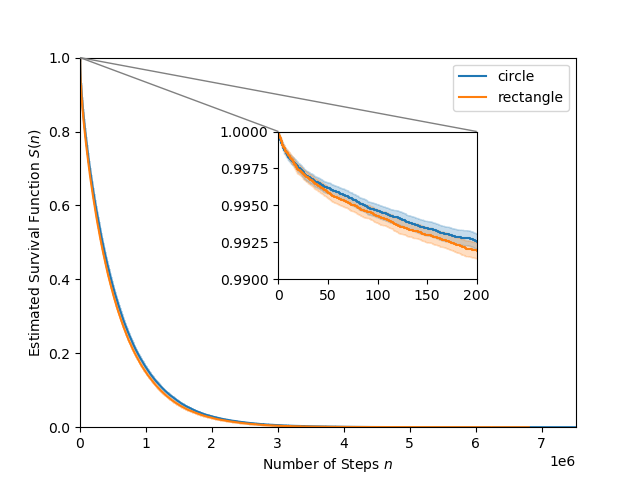
\includegraphics[width=\textwidth]{circle_rect_steps_sf.png}
     \label{fig:sf_simple_shape_steps}
     \caption{}
   \end{figure}


   \begin{table}[h!]
     \centering
     \begin{tabular}{lrr}
        \toprule
         {} &  test\_statistic &             p \\
         \midrule
         Peto & 137.23 & 0.0 \\
         \midrule
         Logrank & 137.23 & 0.0 \\
         \midrule
         Tarone-Ware & 134.31 & 0.0 \\
         \midrule
         Gehan-Breslow & 123.83 & 0.0 \\
         \midrule
         Fleming-Harrington & 123.83 & 0.0 \\
         \bottomrule
     \end{tabular}
     \caption{}
     \label{tab:test_simple_shape_steps}
   \end{table}
   
   

   
   
\subsection{Conclusion}

Given two distinct convex geometries
  \begin{itemize}
     \item the behaviours of the survival function of LRWs are consistent with the theoretical results.
     \item survival curves can be used to describe and distinguish them.
  \end{itemize}
  
